
\chapter{Specifikacija programske potpore}

\section{Funkcionalni zahtjevi}

% Define a counter for use cases
\newcounter{UCCounter}

% Define a command for beginning a new use case
\newcommand{\usecase}[1]{
  \refstepcounter{UCCounter} % Increment the counter
  \noindent\underbar{\textbf{UC\theUCCounter{} - #1}} % Print the use case title with the number
  \begin{packed_item}
}

% Define a command for ending a use case
\newcommand{\closeusecase}{
  \end{packed_item}
  \vspace{1em}
}

\textbf{\textit{dio 1. revizije}}

\textit{ Glavni dionici su bolesnici, djelatnici zdravstvene ustanove te administratori sustava. Bolesnici su krajnji korisnici koji se prijavljuju na rehabilitaciju. Djelatnici zdravstvene ustanove provode rehabilitaciju i upravljaju terminima. Administratori sustava nadziru cjelokupno funkcioniranje sustava i upravljaju korisnicima.}


\noindent \textbf{Dionici:}

\begin{packed_enum}

	\item Administrator
	\item Djelatnik
	\item Bolesnik

\end{packed_enum}

\noindent \textbf{Aktori i njihovi funkcionalni zahtjevi:}


\begin{packed_enum}
	\item  \underbar{Administrator može:}

	\begin{packed_enum}

        \item Prijaviti se u sustav 
	\item Prihvatiti ili odbiti registraciju bolesnika
        \item Pregledati i potvrditi prijave bolesnika za rehabilitaciju
        \item Pregledati sve termine sesija
        \item Dodavati račune djelatnika
        \item Brisati račune bolesnika i djelatnika
        \item Pregledavati, uređivati i brisati podatke računa bolesnika i djelatnika
        \item Otkazati zakazani termin 
        \item Pomicati zakazane termine 

	\end{packed_enum}

	\item  \underbar{Djelatnik može:}

	\begin{packed_enum}

        	\item Prijaviti se u sustav 
		\item Bilježiti napredak svojih bolesnika
		\item Pregledati raspored svojih sesija
		\item Pregledati podatke o bolesnicima
		\item Otkazati sesiju pod određenim uvjetima

	\end{packed_enum}

	\item \underbar{Bolesnik može:}

	\begin{packed_enum}

		\item Registrirati se u sustav
        	\item Prijaviti se u sustav 
		\item Prijaviti se na rehabilitaciju
		\item Odabrati terapiju i termine dolaska na rehabilitaciju
		\item Pomaknuti zakazani termin pod određenim uvjetima
		\item Pregledati vlastiti kalendar s terminima terapije
		\item Pregledati povijest svojih terapija 
  

	\end{packed_enum}

	\item \underbar{Baza podataka:}

	\begin{packed_enum}

		\item Pohranjuje sve podatke o bolesnicima i njihovim rehabilitacijama
		\item Pohranjuje sve potrebne podatke o djelatnicima i njihovim terminima
       		\item Pohranjuje podatke o resursima ustanove 

	\end{packed_enum}
\end{packed_enum}

\eject



\subsection{Obrasci uporabe}

\textbf{\textit{dio 1. revizije}}

\subsubsection{Opis obrazaca uporabe}
\textit{Funkcionalne zahtjeve razraditi u obliku obrazaca uporabe. Svaki obrazac je potrebno razraditi prema donjem predlošku. Ukoliko u nekom koraku može doći do odstupanja, potrebno je to odstupanje opisati i po mogućnosti ponuditi rješenje kojim bi se tijek obrasca vratio na osnovni tijek.}
\vspace{2em} % Dodajte jedan prazan red

\usecase{Zahtjev za registraciju bolesnika u sustav}
	\item \textbf{Glavni sudionik:} Bolesnik
	\item \textbf{Cilj:} Poslati ispravan zahtjev za registraciju u sustav kako bi pristupio procesu rehabilitacije.
	\item \textbf{Sudionici:} Baza podataka
	\item \textbf{Preduvjet:} Bolesnik nema prethodno registriran korisnički račun
	\item \textbf{Opis osnovnog tijeka:}
	\begin{packed_enum}
		\item Bolesnik unosi osobne podatke, adresu elektroničke pošte i lozinku.
	\end{packed_enum}
\closeusecase


\usecase{Potvrda registracije bolesnika u sustav}
	\item \textbf{Glavni sudionik:} Administrator
	\item \textbf{Cilj:} Provjeriti i potvrditi registraciju bolesnika.
	\item \textbf{Sudionici:} Baza podataka, Bolesnik
	\item \textbf{Preduvjet:} Bolesnik je prethodno poslao zahtjev za registraciju, administrator je prijavljen u sustav.
	\item \textbf{Opis osnovnog tijeka:}
	\begin{packed_enum}
		\item Administrator provjerava ispravnost podataka.
		\item Sustav pohranjuje podatke i stvara korisnički račun.
  		\item Bolesnik prima elektroničku poštu s potvrdom registracije.
	\end{packed_enum}
	\item \textbf{Opis mogućih odstupanja:}
	U slučaju neispravne registracije u smislu duplikata OIB-a ili MBO-a frontend ne dopušta slanje registracije. 
    	Ukoliko nepravilnosti uoči administrator, Bolesnik prima elektroničku poštu na upisanu adresu u kojoj mu se govori da registracija nije uspjela.
\closeusecase


\usecase{Prijava bolesnika/djelatnika/administratora u sustav}
	\item \textbf{Glavni sudionik:} Bolesnik/Djelatnik/Administrator
	\item \textbf{Cilj:} Korisnik se želi prijaviti u sustav 
	\item \textbf{Sudionici:} Baza podataka
	\item \textbf{Preduvjet:} Korisnikov račun je u bazi podataka
	\item \textbf{Opis osnovnog tijeka:}
	\begin{packed_enum}
		\item Korisnik unosi adresu elektroničke pošte i lozinku.
		\item Provjerava se postojanost dane kombinacije u bazi
		\item Ovisno o tipu profila povezanog s unesenim podacima, korisniku se otvara jedno od 3 moguća sučelja (bolesnik, djelatnik, administrator)
	\end{packed_enum}
	\item \textbf{Opis mogućih odstupanja:}
	Sustav reagira na neispravne podatke te obavještava korisnika o netočnosti podataka. \\
\closeusecase


\usecase{Zaboravljena lozinka za prijavu}
	\item \textbf{Glavni sudionik:} Bolesnik/Djelatnik/Administrator
 	\item \textbf{Cilj:} Prijaviti se unatoč zaboravljenoj lozinci
  	\item \textbf{Sudionici:} Baza podataka
   	\item \textbf{Preduvjet:} Korisnikova e-mail adresa je u bazi podataka
    	\item \textbf{Opis osnovnog tijeka:}
     	\begin{packed_enum}
      		\item Korisnik je zaboravio lozinku te se ne može prijaviti u sustav
		\item Korisnik pritišće gumb za dobivanje nove lozinke
  		\item Korisnik na e-mail adresu dobiva upute za postavljanje nove lozinke
    	\end{packed_enum}
\closeusecase


\usecase{Prijava bolesnika na rehabilitaciju}
	\item \textbf{Glavni sudionik:} Bolesnik
	\item \textbf{Cilj:} Prijaviti se za proces rehabilitacije.
	\item \textbf{Sudionici:} Baza podataka
	\item \textbf{Preduvjet:} Bolesnik je registriran i prijavljen u sustav.
	\item \textbf{Opis osnovnog tijeka:}
	\begin{packed_enum}
		\item Bolesnik odabire opciju za prijavu na rehabilitaciju.
		\item Bolesnik unosi informacije o svom oboljenju, potrebnom postupku liječenja i liječniku koji ga je uputio na rehabilitaciju.
        	\item S obzirom na unesenu vrstu rehabilitacije, sustav provjerava koji su sve termini slobodni (slobodan termin: slobodan resurs i slobodan specijalizirani djelatnik) 
		\item Bolesnik odabire datum i vrijeme svojih termina na temelju dostupnih termina 
        	\item Bolesnik čeka odobrenje administratora (UC18) 
        	\item Korisnik prima skočni prozor s obavijesti o administratorovoj odluci te sukladno istoj ili može ponoviti prijavu na rehabilitaciju ili je preusmjeren na kontrolnu ploču (dashboard) za novonastalu rehabilitaciju
	\end{packed_enum}
	\item \textbf{Opis mogućih odstupanja:}
	Dok sve nužne informacije nisu upisane blokirano je slanje forme na provjeru kod administratora. 
    Korisniku nije dopušteno odabrati sesije koje su vremenski udaljene manje od minimalne razlike između dvije sesije koja je definirana terapijom. 
    Korisniku nije dopušteno slanje forme ukoliko je vremenska razlika između zadnje i prve sesije duža od maksimalnog trajanja terapije koje je definirano terapijom.
\closeusecase


\usecase{Promjena zakazanog termina (bolesnik)}
	\item \textbf{Glavni sudionik:} Bolesnik
	\item \textbf{Cilj:} Promijeniti zakazani termin za rehabilitaciju.
	\item \textbf{Sudionici:} Baza podataka
	\item \textbf{Preduvjet:} Bolesnik je registriran, prijavljen i ima zakazane termine.
	\item \textbf{Opis osnovnog tijeka:}
	\begin{packed_enum}
        	\item Bolesnik ulazi na kontrolnu ploču.
	 	\item Bolesnik pregledava svoj raspored i odabire termin koji bi htio promijeniti.
		\item Bolesnik u informacijama o terminu odabire opciju za promjenu termina.
		\item Bolesnik pregledava raspored slobodnih termina i odabire zamjenski termin.
		\item Sustav potvrđuje regularnost promjene i ona se evidentira na kontrolnoj ploči djelatnika i bolesnika. 
	\end{packed_enum}
    	\item \textbf{Opis mogućih odstupanja:}
		Ako promjena nije napravljena minimalno 48 sati prije termina, otkazivanja su onemogućena u sustavu i bolesnik se upućuje da u slučaju hitnosti kontaktira administratora direktno. 
\closeusecase


\usecase{Pregled relevantnih informacija za budući termin}
	\item \textbf{Glavni sudionik:} Bolesnik
 	\item \textbf{Cilj:} Dobiti više informacija o određenom terminu
  	\item \textbf{Sudionici:} Baza podataka
   	\item \textbf{Preduvjet:} Korisnik je prijavljen u sustav, prijavljen na terapiju i ima barem jedan preostali termin
    	\item \textbf{Opis osnovnog tijeka:}
     	\begin{packed_enum}
      		\item Korisnik na svojem rasporedu odabire jedan termin
		\item Korisnik pritišće gumb "Prikaži više" za taj termin
  		\item Korisniku se pojavljuje novi prozor s informacijama o terminu kao što su broj sesije, opis sesije, ime djelatnika te mapa ustanove s naznačenim mjestom odvijanja te sesije
    	\end{packed_enum}
\closeusecase


\usecase{Otkazivanje zakazanog termina (djelatnik)}
	\item \textbf{Glavni sudionik:} Djelatnik
	\item \textbf{Cilj:} Otkazati zakazani termin za rehabilitaciju.
	\item \textbf{Sudionici:} Baza podataka
	\item \textbf{Preduvjet:} Djelatnik je prijavljen u sustav. Bolesnik ima zakazane termine.
	\item \textbf{Opis osnovnog tijeka:}
	\begin{packed_enum}
        	\item Djelatnik ulazi na kontrolnu ploču i odabire termin koji želi promijeniti.
		\item Djelatnik odabire opciju za otkazivanje termina 
        	\item Izvršava se promjena u bazi te se obavještava bolesnik koji odabire novi termin 
	\end{packed_enum}
    \item \textbf{Opis mogućih odstupanja:}
	Djelatnik ne može otkazivati termine koji nisu njegovi. 
\closeusecase


\usecase{Otkazivanje zakazanog termina (administrator)}
	\item \textbf{Glavni sudionik:} Administrator
	\item \textbf{Cilj:} Otkazati zakazani termin za rehabilitaciju.
	\item \textbf{Sudionici:} Baza podataka
	\item \textbf{Preduvjet:} Administrator je prijavljen u sustav. Bolesnik ima zakazane termine.
	\item \textbf{Opis osnovnog tijeka:}
	\begin{packed_enum}
        	\item Administrator odlazi na kalendar i pretražuje termin po djelatniku i/ili po bolesniku.
		\item Administrator odabire opciju za otkazivanje termina 
        	\item Izvršava se promjena u bazi te se obavještava djelatnika i bolesnika koji odabire novi termin 
	\end{packed_enum}
\closeusecase


\usecase{Pregled kalendara vlastitih terapija}
	\item \textbf{Glavni sudionik:} Bolesnik/Djelatnik
	\item \textbf{Cilj:} Pregledati kalendar s terminima terapije.
	\item \textbf{Sudionici:} Baza podataka
	\item \textbf{Preduvjet:} Bolesnik/Djelatnik je registriran i prijavljen u sustav.
	\item \textbf{Opis osnovnog tijeka:}
	\begin{packed_enum}
		\item Bolesnik/Djelatnik odabire opciju za pregled vlastitog kalendara.
		\item Sustav prikazuje raspored svih zakazanih termina terapije.
        	\item Bolesnik može pregledati sesije i vidjeti napomene, djelatnik ih može upisivati
	\end{packed_enum}
\closeusecase


\usecase{Pregled podataka o bolesnicima}
	\item \textbf{Glavni sudionik:} Djelatnik
	\item \textbf{Cilj:} Pregledati podatke o bolesnicima.
	\item \textbf{Sudionici:} Baza podataka
	\item \textbf{Preduvjet:} Djelatnik je prijavljen u sustav.
	\item \textbf{Opis osnovnog tijeka:}
	\begin{packed_enum}
		\item Djelatnik pretražuje ime bolesnika ili pregledava listu svih bolesnika.
		\item Sustav prikazuje popis bolesnika i osnovne informacije o njima.
		\item Djelatnik može pregledati detaljnije podatke o svakom bolesniku.
	\end{packed_enum}
\closeusecase


\usecase{Pregled rasporeda svih bolesnika, djelatnika i sesija}
	\item \textbf{Glavni sudionik:} Administrator
	\item \textbf{Cilj:} Pregledati raspored bolesnika i sesija rehabilitacije.
	\item \textbf{Sudionici:} Baza podataka
	\item \textbf{Preduvjet:} Administrator je prijavljen u sustav.
	\item \textbf{Opis osnovnog tijeka:}
	\begin{packed_enum}
		\item Administrator odabire opciju za pregled rasporeda.
		\item Sustav prikazuje raspored svih bolesnika, djelatnika i sesija.
		\item Administrator može filtrirati raspored po različitim kriterijima.
	\end{packed_enum}
\closeusecase


\usecase{Bilježenje napretka bolesnika}
	\item \textbf{Glavni sudionik:} Djelatnik
	\item \textbf{Cilj:} Bilježiti i evidentirati napredak bolesnika tijekom procesa rehabilitacije.
	\item \textbf{Sudionici:} Baza podataka
	\item \textbf{Preduvjet:} Bolesnik je registriran, prijavljen i odradio sesiju rehabilitacije s određenim djelatnikom.
	\item \textbf{Opis osnovnog tijeka:}
	\begin{packed_enum}
		\item Djelatnik odabire bolesnika za bilježenje napretka.
		\item Djelatnik unosi podatke o sesiji rehabilitacije.
		\item Djelatnik potvrđuje unos i sprema podatke.
	\end{packed_enum}
\closeusecase


\usecase{Pregled podataka o terapijama}
	\item \textbf{Glavni sudionik:} Bolesnik
	\item \textbf{Cilj:} Pregledati podatke o terapijama.
	\item \textbf{Sudionici:} Baza podataka
	\item \textbf{Preduvjet:} Bolesnik je registriran i prijavljen u sustav.
	\item \textbf{Opis osnovnog tijeka:}
	\begin{packed_enum}
		\item Bolesnik odabire opciju za pregled podataka.
		\item Sustav prikazuje relevantne informacije o terapijama.
	\end{packed_enum}
\closeusecase


\usecase{Pregled statistike o djelatnicima i resursima}
	\item \textbf{Glavni sudionik:} Administrator 
	\item \textbf{Cilj:} Praćenje dostupnosti osoblja, opreme i kapaciteta za rehabilitaciju.
	\item \textbf{Sudionici:} Baza podataka
	\item \textbf{Preduvjet:} Administrator je prijavljen u sustav.
	\item \textbf{Opis osnovnog tijeka:}
	\begin{packed_enum}
		\item Administrator iz kontrolne ploče odabire Pregled statistike o djelatnicima i resursima
		\item Sustav prikazuje zadani pogled (engl. \textit{view}). 
	\end{packed_enum}
\closeusecase


\usecase{Dodavanje djelatnika u bazu}
	\item \textbf{Glavni sudionik:} Administrator
	\item \textbf{Cilj:} Stvoriti korisnički račun za novog djelatnika u sustavu medicinske rehabilitacije.
	\item \textbf{Sudionici:} Baza podataka
	\item \textbf{Preduvjet:} Administrator je prijavljen u sustav.
	\item \textbf{Opis osnovnog tijeka:}
	\begin{packed_enum}
		\item Administrator iz kontrolne ploče odabire opciju za stvaranje novog djelatnika.
		\item Sustav prikazuje obrazac za unos osobnih podataka novog djelatnika.
		\item Administrator unosi sve potrebne podatke o novom djelatniku.
		\item Ako su svi podaci ispravni, sustav stvara novi korisnički račun za djelatnika.
	\end{packed_enum}
	\item \textbf{Opis mogućih odstupanja:}
	Sustav reagira na neispravne podatke, već postojeće zaposlenike te obavještava administratora o neuspjelom upisu.
\closeusecase


\usecase{Promjena podataka o djelatnicima i bolesnicima}
	\item \textbf{Glavni sudionik:} Administrator
	\item \textbf{Cilj:} Izmijeniti informacije o djelatnicima i bolesnicima u bazi.
	\item \textbf{Sudionici:} Baza podataka
	\item \textbf{Preduvjet:} Administrator je prijavljen u sustav.
	\item \textbf{Opis osnovnog tijeka:}
	\begin{packed_enum}
		\item Administrator iz kontrolne ploče odabire pregled svih djelatnika ili bolesnika.
		\item Administrator odabire djelatnika/bolesnika i uređuje informacije o istom.
        	\item Prije potvrde o promjeni administrator ponovno unosi svoju šifru
	\end{packed_enum}
\closeusecase


\usecase{Potvrda o ispravnoj prijavi na rehabilitaciju}
	\item \textbf{Glavni sudionik:} Administrator
 	\item \textbf{Cilj:} Potvrditi bolesnikovu prijavu na određenu rehabilitaciju
  	\item \textbf{Sudionici:} Baza podataka
   	\item \textbf{Preduvjet:} Administrator je prijavljen u sustav i bolesnik je predao zahtjev za prijavu na rehabilitaciju
    	\item \textbf{Opis osnovnog tijeka:}
     	\begin{packed_enum}
      		\item Administrator je obaviješten kako je dobio novi zahtjev za prijavu
		\item Administrator analizira podatke o bolesniku i o prijavi te zajedno s informacijama iz baze podataka donosi odluku o ispravnosti zahtjeva
  		\item S obzirom na rezultat svoje odluke, administrator ili omogućuje prijavu na rehabilitaciju ili dojavljuje bolesniku poruku o pogrešci
    	\end{packed_enum}
\closeusecase


\usecase{Deaktivacija korisničkog računa djelatnika/bolesnika}
	\item \textbf{Glavni sudionik:} Administrator
	\item \textbf{Cilj:} Deaktivirati korisnički račun djelatnika/bolesnika.
	\item \textbf{Sudionici:} Baza podataka
	\item \textbf{Preduvjet:} Administrator je prijavljen u sustav.
	\item \textbf{Opis osnovnog tijeka:}
	\begin{packed_enum}
		\item Administrator iz kontrolne ploče odabire pregled svih djelatnika ili bolesnika.
		\item Administrator odabire djelatnika/bolesnika čiji korisnički račun želi deaktivirati.
        	\item Prije potvrde o promjeni administrator ponovno unosi svoju šifru
	\end{packed_enum}
\closeusecase


\usecase{Deaktivacija vlastitog korisničkog računa}
	\item \textbf{Glavni sudionik:} Bolesnik
	\item \textbf{Cilj:} Deaktivirati vlastiti korisnički račun.
	\item \textbf{Sudionici:} Baza podataka
	\item \textbf{Preduvjet:} Bolesnik je prijavljen u sustav.
	\item \textbf{Opis osnovnog tijeka:}
	\begin{packed_enum}
		\item Bolesnik odabire opciju za deaktivaciju računa.
		\item Sustav traži bolesnikovu lozinku za potvrdu zahtjeva.
		\item Sustav je deaktivirao bolesnikov korisnički račun.
	\end{packed_enum}
	\item \textbf{Opis mogućih odstupanja:}
	Sustav reagira na neispravnu lozinku te obavještava bolesnika o neuspjelom pokušaju.
\closeusecase


\vspace{2cm}

\subsubsection{Dijagrami obrazaca uporabe}


\begin{figure}[h]
    \centering
    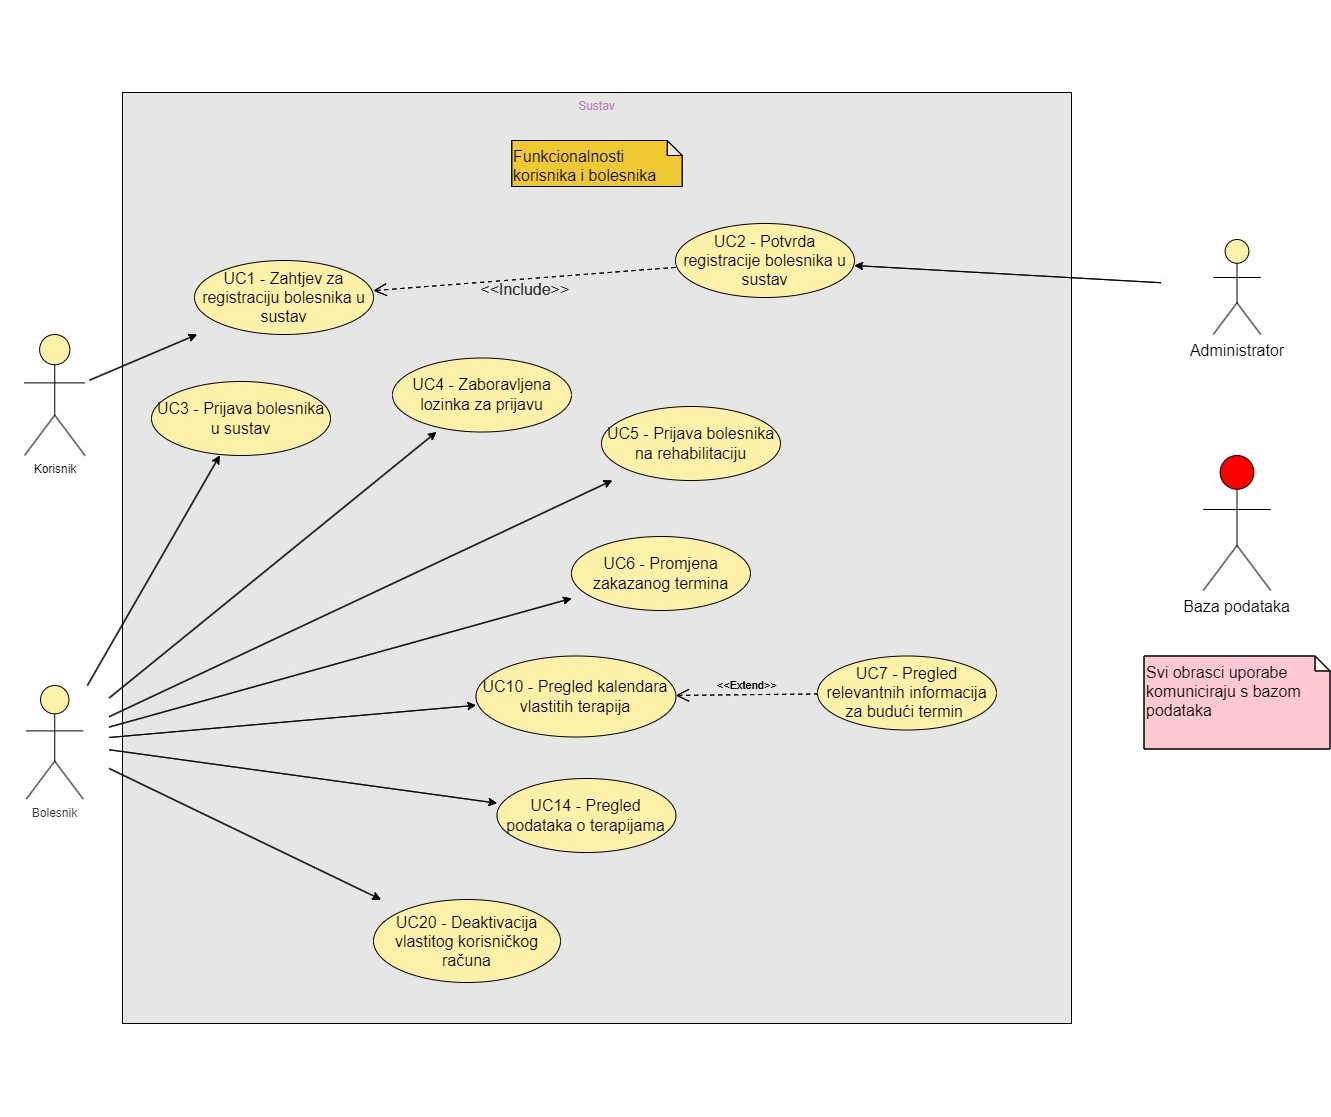
\includegraphics[width=\textwidth]{./slike/UC Dijagram - Bolesnik} 
    \caption{Dijagram obrasca uporabe, funkcionalnost bolesnika}
    \label{fig:my_image}
\end{figure}

\begin{figure}[bp]
    \centering
    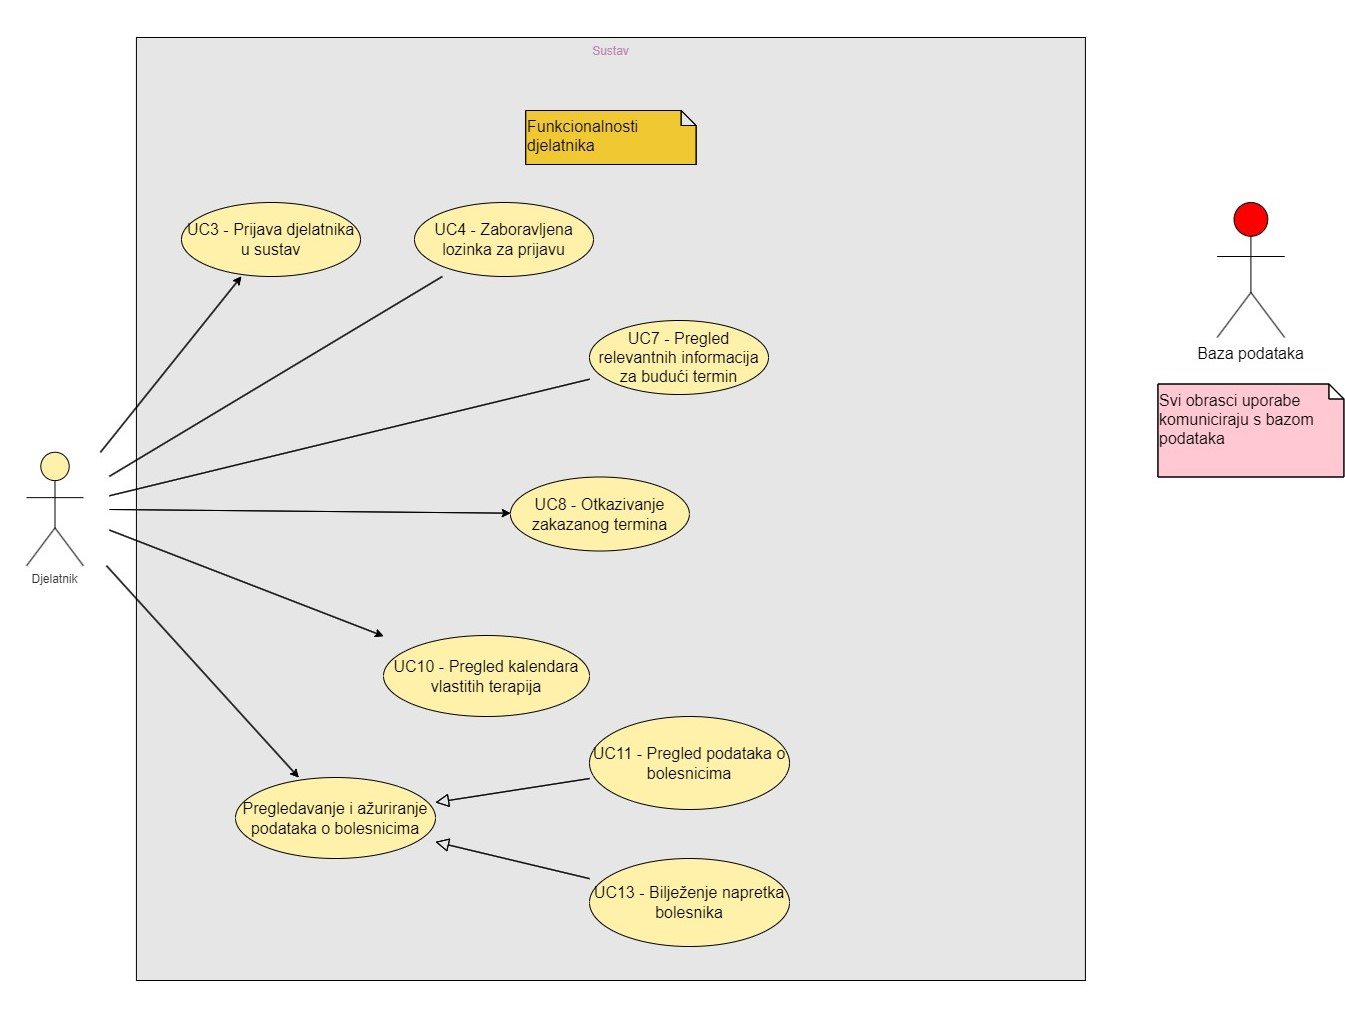
\includegraphics[width=\textwidth]{./slike/UC Dijagram - Djelatnik} 
    \caption{Dijagram obrasca uporabe, funkcionalnost djelatnika}
    \label{fig:my_image}
\end{figure}

\begin{figure}[bp]
    \centering
    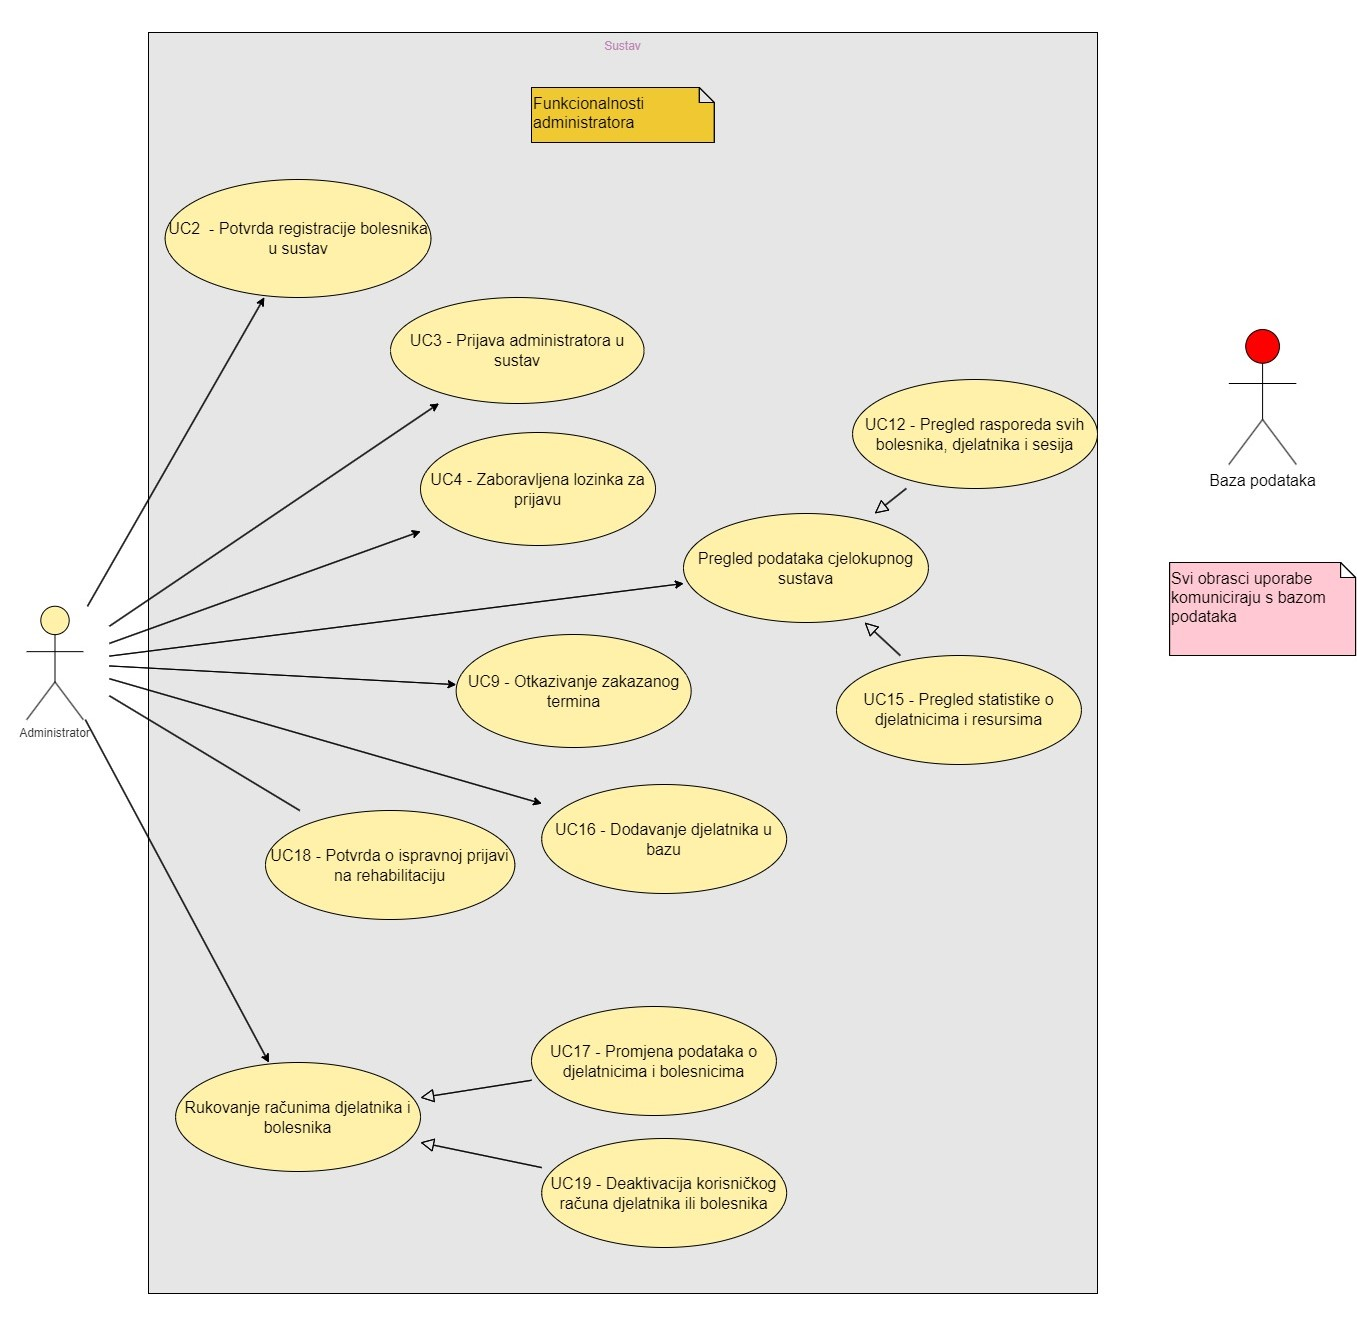
\includegraphics[width=\textwidth]{./slike/UC Dijagram - Administrator} 
    \caption{Dijagram obrasca uporabe, funkcionalnost administratora}
    \label{fig:my_image}
\end{figure}
\eject

\subsection{Sekvencijski dijagrami}

\textbf{\textit{dio 1. revizije}}\\



\textbf{Obrazac uporabe UC5 – Prijava bolesnika na rehabilitaciju}

Za prijavu na rehabilitaciju, bolesnik pritišće na gumb s kojim dobiva od web aplikacije prikaz za prijavu te zatim unosi sve podatke o rehabilitaciji na koju se želi prijaviti. Te informacije se šalju bazi kako bi se provjerile te se, ako nije došlo do pogreške, vraćaju svi slobodni termini koje onda web aplikacija koristi za kreaciju kalendara slobodnih termina i to prikazuje bolesniku. Zatim, bolesnik mora odabrati onoliko termina koliko je naveo u prijavi te odabire svoje termine sve dok ne odabere toliko točnih termina. Svaki termin je određen svojim datumom i vremenom, jednom kada bolesnik odabere jedan termin, u bazi se provjerava slijedi li taj termin sva pravila (postoji minimalan razmak među terminima koji se mora poštovati) te ako odabrani termin nije valjan, sustav bolesniku vraća odgovarajuću poruku, a taj se termin ne uzima u obzir. Ako je termin valjan, bolesnik može prijeći na izabiranje sljedećeg termina. Na kraju, kada je bolesnik odabrao točan broj valjanih termina, svi termini se šalju i zapisuju u bazu, a bolesniku se ispisuje poruka kako mora pričekati potvrdu administratora sustava.

\begin{figure}[h!]
    \centering
    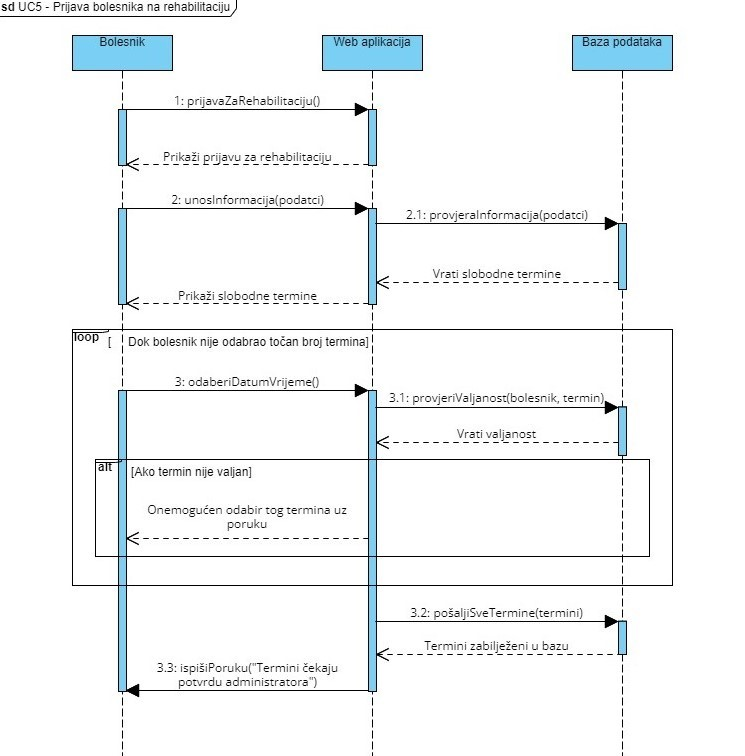
\includegraphics[width=\textwidth]{./slike/Sekvencijski - UC5.jpg} 
    \caption{Sekvencijski dijagram za UC5}
    \label{fig:my_image}
\end{figure}
\eject


\textbf{Obrazac uporabe UC6 – Promjena zakazanog termina}

Bolesnik pritiskom na odgovarajući gumb dobiva prikaz svojeg raspored koji aplikacija dohvaća iz baze te na tom rasporedu odabire termin koji mu je dodijeljen, a koji bi želio promijeniti. Pojavljuju se dodatne informacije o odabranom terminu i također gumb za mijenjanje termina, pritiskom na taj gumb, web aplikacija dohvaća sve moguće termine zamjene za tog bolesnika i za tu rehabilitaciju i prikazuje ih bolesniku. Od ponuđenih termina, bolesnik odabire jedan te web aplikacija obavlja zamjenu u bazi podataka. Ako je zamjena prošla bez pogrešaka, promjena se odmah evidentira na kontrolnoj ploči dok u suprotnom bolesniku dolazi poruka o pogrešci.



\begin{figure}[h!]
    \centering
    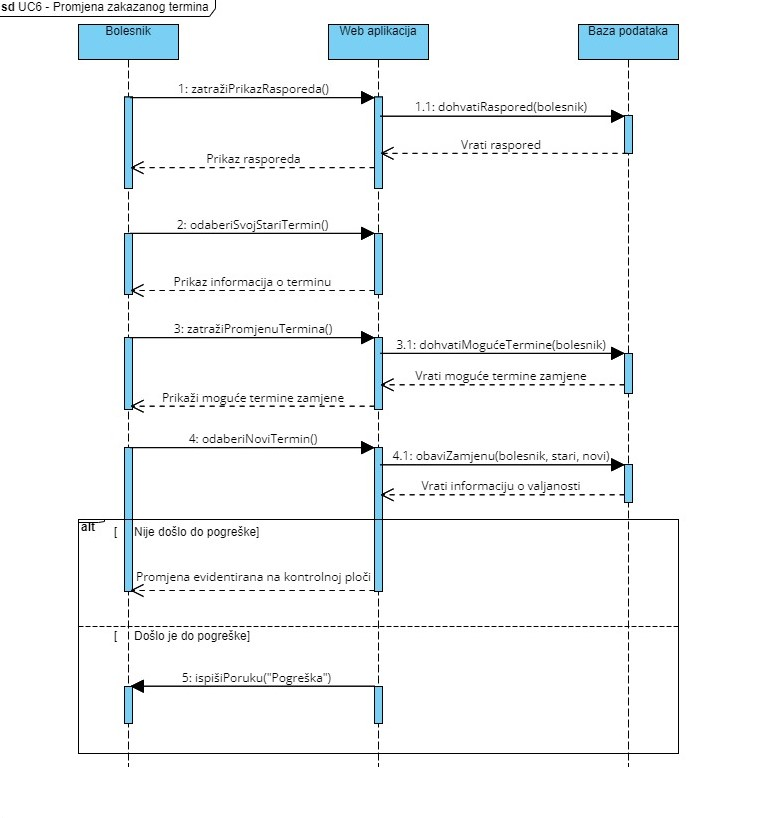
\includegraphics[width=\textwidth]{./slike/Sekvencijski - UC6.jpg} 
    \caption{Sekvencijski dijagram za UC6}
    \label{fig:my_image}
\end{figure}
\eject

\textbf{Obrazac uporabe UC13 – Bilježenje napretka bolesnika}

Djelatnik odabire bolesnika kojem želi zabilježiti napredak, a sustav vraća iz baze dohvaćene podatke o tom bolesniku. Djelatnik zatim piše svoj zapis o napretku, a kada završi, sustav od njega traži potvrdu. Jednom kada djelatnik potvrdi svoj zapis, web aplikacija ga šalje bazi podataka gdje se i upisuje.
genijalan i prekoristan sekvencijski dijagram.

\begin{figure}[h!]
    \centering
    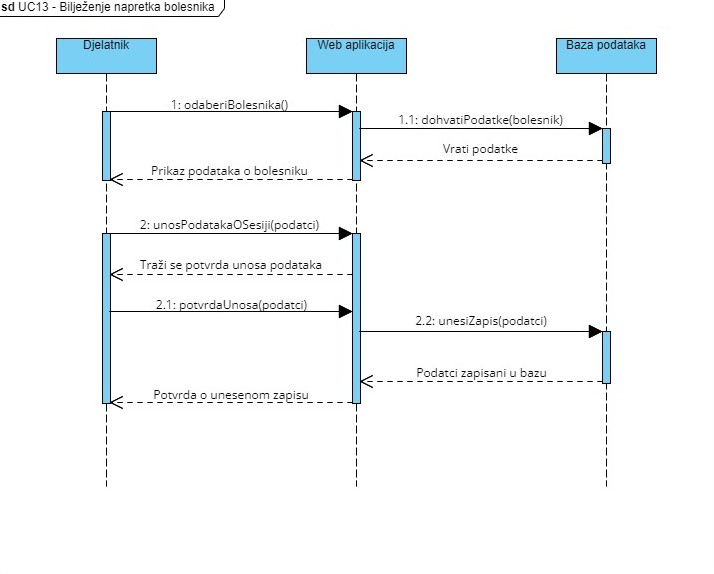
\includegraphics[width=\textwidth]{./slike/Sekvencijski - UC13.jpg} 
    \caption{Sekvencijski dijagram za UC13}
    \label{fig:my_image}
\end{figure}
\eject

\textbf{Obrazac uporabe UC16 - Dodavanje djelatnika u bazu}

Administrator odabire prikaz za stvaranje novog djelatnika, a web aplikacija mu ga vraća. Administrator zatim unosi sve podatke novog djelatnika kojeg želi dodati u sustav te se ti podatci s web aplikacije šalju bazi podataka. Baza podataka tada, ako nije došlo do pogreške, dodaje novog djelatnika u sustav, ako je do pogreške slučajno došlo, administrator se odgovarajućom porukom obavještava o njoj.

\begin{figure}[h!]
    \centering
    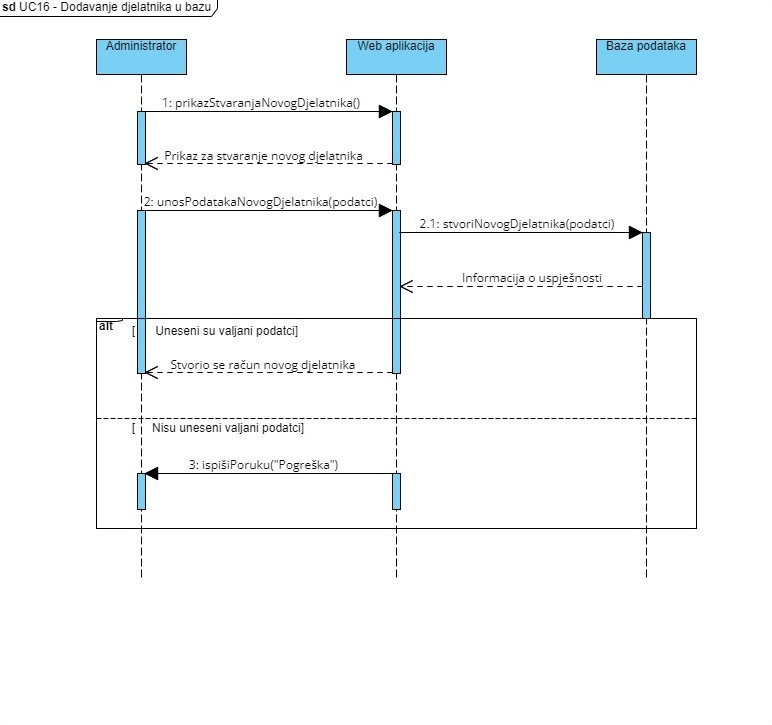
\includegraphics[width=\textwidth]{./slike/Sekvencijski - UC16.jpg} 
    \caption{Sekvencijski dijagram za UC16}
    \label{fig:my_image}
\end{figure}
\eject

\section{Ostali zahtjevi}


\textbf{\textit{dio 1. revizije}}\\

\textit{Nefunkcionalni zahtjevi i zahtjevi domene primjene ključni su za uspješno funkcioniranje našeg sustava. Oni definiraju kako se sustav treba ponašati, koje standarde kvalitete mora zadovoljiti, te koje sigurnosne i tehničke ograničenja treba poštivati.}

\subsection*{Performanse i pouzdanost}
\begin{itemize}
    \item Sustav treba podržavati simultani rad više korisnika bez gubitka performansi, osiguravajući pouzdano iskustvo u stvarnom vremenu.
    \item Vrijeme odziva prilikom pristupa bazi podataka i drugim ključnim funkcijama sustava ne smije trajati duže od nekoliko sekundi. Time se osigurava brz i efikasan rad sustava.
\end{itemize}

\subsection*{Korisničko iskustvo}
\begin{itemize}
    \item Korisničko sučelje treba biti intuitivno i jednostavno za korištenje, uz minimalnu potrebu za opsežnim instrukcijama ili obukom.
    \item Sustav mora podržavati više jezika i odgovarajuće posebne znakove u različitim jezicima (starija populacija govori samo materinjim jezikom i sl.). Prva verzija aplikacije bit će na engleskom. 
    \item Neispravno korištenje korisničkog sučelja ne smije narušiti funkcionalnost i rad sustava.
\end{itemize}

\subsection*{Sigurnost i zaštita podataka}
\begin{itemize}
    \item Sustav mora osigurati visoku razinu sigurnosti, koristeći enkripciju i druge sigurnosne protokole, posebice u komunikaciji s bazom podataka i tijekom prijenosa osjetljivih podataka.
    \item Pristup sustavu mora biti omogućen kroz sigurne protokole kao što je HTTPS čime se osigurava zaštita podataka i privatnosti korisnika.
\end{itemize}

\subsection*{Platforma i tehnička implementacija}
\begin{itemize}
    \item Sustav će biti implementiran kao web aplikacija, koristeći objektno-orijentirane jezike, što omogućuje fleksibilnost i lakše održavanje.
    \item Aplikacija treba biti prilagodljiva i kompatibilna s različitim web i mobilnim platformama, osiguravajući široku dostupnost i pristupačnost.
\end{itemize}

\subsection*{Skalabilnost i nadogradnje}
\begin{itemize}
    \item Sustav mora biti skalabilan kako bi podržao rast broja korisnika i povećanje opterećenja bez gubitka performansi.
    \item Nadogradnje sustava trebaju biti implementirane na način da ne narušavaju postojeće funkcionalnosti i da se mogu efikasno integrirati u operativni sustav.
\end{itemize}

\subsection*{Standardi Kvalitete i usklađenost}
\begin{itemize}
\item Sustav treba biti usklađen s nacionalnim i međunarodnim standardima kvalitete i sigurnosti, uključujući regulative vezane za zdravstvene informacijske sustave.
\item Redovite provjere kvalitete i revizije trebaju osigurati da aplikacija kontinuirano zadovoljava sve postavljene standarde.
\end{itemize}

\subsection*{Dostupnost i pouzdanost}
\begin{itemize}
\item Sustav treba osigurati visoku dostupnost i minimalno vrijeme prekida, posebno tijekom radnih sati zdravstvenih ustanova.
\item Plan oporavka u slučaju kvara ili prekida treba biti jasno definiran i implementiran, osiguravajući brz povratak u normalan rad.
\end{itemize}

\subsection*{Pristupačnost i inkluzivnost}
\begin{itemize}
\item Sustav treba biti dizajniran s obzirom na pristupačnost, omogućavajući laku upotrebu osobama s različitim stupnjevima sposobnosti, uključujući stariju populaciju i osobe s invaliditetom.
\item Također, treba podržavati prilagodbe za korisnike s posebnim potrebama poput prilagođenih fontova, kontrasta i pomoćnih tehnologija.
\end{itemize}

\subsection*{Interoperabilnost i integracija}
\begin{itemize}
    \item Sustav treba biti interoperabilan s drugim zdravstvenim informacijskim sustavima, omogućujući razmjenu podataka i integraciju s postojećim IT infrastrukturama.
    \item Integracija s vanjskim API-ima i servisima treba biti omogućena za proširivanje funkcionalnosti sustava kao što su integracije s laboratorijskim sustavima, elektroničkim zdravstvenim kartonima i slično.
\end{itemize}

\subsection*{Održivost i ekološka osjećajnost}
\begin{itemize}
    \item Sustav treba biti razvijen s obzirom na ekološke aspekte, promovirajući smanjenje upotrebe papira i drugih materijala u zdravstvenim ustanovama.
    \item Digitalizacija procesa treba doprinijeti održivijem načinu rada, smanjujući otpad i potrebu za fizičkim resursima.
\end{itemize}

\subsection*{Prilagodba zakonodavnim okvirima}
\begin{itemize}
    \item Sustav treba biti u skladu s lokalnim i međunarodnim zakonodavnim okvirima, uključujući propise o zaštiti osobnih podataka (npr. GDPR u EU).
    \item Moraju se implementirati mehanizmi za usklađenost s pravnim zahtjevima u vezi sa zdravstvenim informacijama kao što su prava na pristup, ispravak i brisanje osobnih podataka.
\end{itemize}

\subsection*{Praćenje i izvještavanje}
\begin{itemize}
    \item Sustav treba omogućiti generiranje detaljnih izvještaja o korištenju resursa, učinkovitosti i performansama procesa rehabilitacije.
    \item Treba biti omogućeno praćenje korištenja aplikacije, uključujući analitiku i povratne informacije od korisnika za kontinuirano poboljšanje i prilagodbu sustava.
\end{itemize}

\subsection*{Prilagodljivost budućim tehnološkim trendovima}
\begin{itemize}
    \item Sustav treba biti dizajniran s mogućnošću laganog ažuriranja i prilagodbe novim tehnološkim trendovima i inovacijama.
    \item Treba postojati mogućnost integracije s budućim tehnologijama poput umjetne inteligencije, strojnog učenja i napredne analitike podataka.
\end{itemize}


\eject

